\section{OCR Systems: Promises and Pitfalls}
\label{sec:analysis}
As briefly alluded to in the introduction, training an OCR model for each endangered language is challenging, given the limited available data. 
Instead, we use the general-purpose OCR system from the Google Vision AI toolkit\footnote{\url{https://cloud.google.com/vision}} to get the first pass OCR transcription on our data.

The Google Vision OCR system~\cite{fujii2017sequence,ingle2019scalable} is highly performant and supports 60 major languages in 29 scripts. It can transcribe a wide range of higher resource languages with high accuracy, ideal for our proposed method of incorporating high-resource translations into the post-correction model. Moreover, it is particularly well-suited to our task because it provides script-specific OCR models in addition to language-specific ones. Per-script models are more robust to unknown languages because they are trained on data from multiple languages and can act as a general character recognizer without relying on a single language's model. Since most endangered languages adopt standard scripts (often from the region's dominant language) as their writing systems, the per-script recognition models can provide a stable starting point for post-correction.

The metrics we use for evaluating performance are character error rate (CER) and word error rate (WER), representing the ratio of erroneous characters or words in the OCR prediction to the total number in the annotated transcription. More details are in \autoref{sec:experiments}. The CER and WER using the Google Vision OCR on our dataset are in \autoref{tab:google_metrics}.

\subsection{OCR Performance}
\begin{table}[tb]
    \centering
    \small
    \begin{tabular}{lcrr}
    \toprule
    Language && CER & WER \\
    \midrule
    Ainu && 1.34 & 6.27 \\
    Griko && 3.27 & 15.63 \\
    Yakkha && 8.90 & 31.64 \\
    \bottomrule
    \end{tabular}
    \caption{Character error rate and word error rate with the Google Vision OCR system on our dataset.}
    \label{tab:google_metrics}
\end{table}
Across the three languages, the error rates indicate that we have a first pass transcription that is of reasonable quality, giving our post-correction method a reliable starting point. We note the particularly low CER for the Ainu data, reflecting previous work that has evaluated the Google Vision system to have strong performance on typed Latin script documents \cite{fujii2017sequence}. However, there remains considerable room for improvement in both CER and WER for all three languages.

Next, we look at the edit distance between the predicted and the gold transcriptions, in terms of insertion, deletion, and replacement operations. Replacement accounts for over 84\% of the errors in the Griko and Ainu datasets, and 55\% overall. This pattern is expected in the OCR task, as the recognition model uses the image to make predictions and is more likely to confuse a character's shape for another than to hallucinate or erase pixels. However, we observe that the errors in the Yakkha dataset do not follow this pattern. Instead, 87\% of the errors for Yakkha occur because of deleted characters.

\subsection{Types of Errors}

\begin{figure}[t]
    \centering
    \small
    \begin{tabular}{ccc}
        \frame{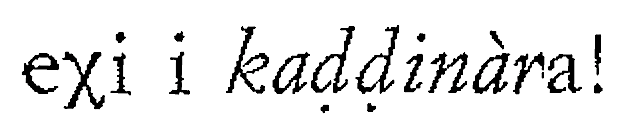
\includegraphics[width=0.4\columnwidth]{images/errors1a.pdf}} & \raisebox{0.7em}{$\xrightarrow{\mathrm{OCR}}$} & \raisebox{0.7em}{\large e\textcolor{burntred}{\textbf{x}}i i ka\textcolor{burntred}{\textbf{dd}}in\`ara} \\[.1cm]
        \frame{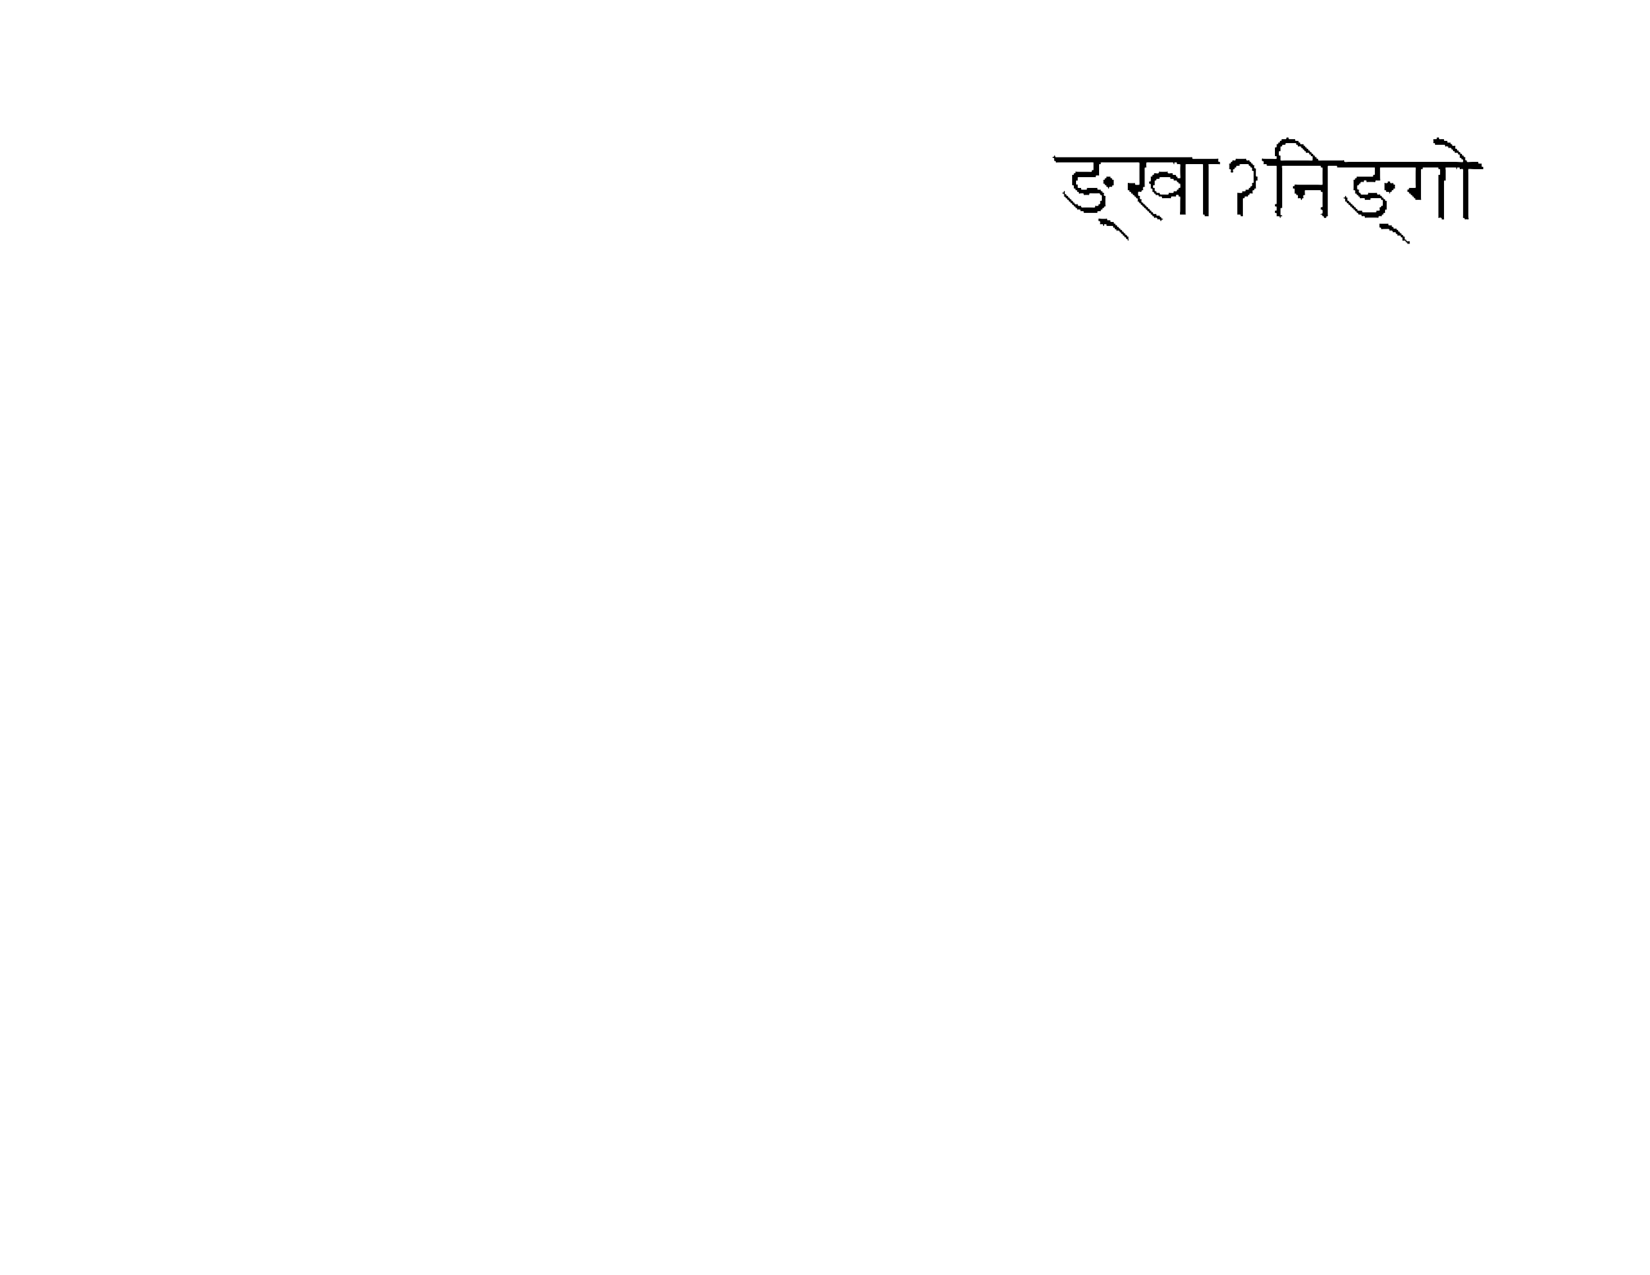
\includegraphics[width=0.3\columnwidth]{images/errors2a.pdf}} &
        \raisebox{0.6em}{$\xrightarrow{\mathrm{OCR}}$} &
        
\includegraphics[width=0.3\columnwidth]{images/error2b.pdf} \\
    \end{tabular}
    \caption{Examples of errors in Griko (top) and Yakkha (bottom) when using the Google Vision OCR.}
    \label{fig:ocr_errors}
\end{figure}

To better understand the challenges posed by the endangered language setting, we manually inspect all the errors made by the OCR system. While some errors are commonly seen in the OCR task, such as misidentified punctuation or incorrect word boundaries, 85\% of the total errors occur due to specific characteristics of endangered languages that general-purpose OCR systems do not account for. Broadly, they can be categorized into two types, examples of which are shown in \autoref{fig:ocr_errors}:
\begin{itemize}[leftmargin=*, itemsep=2pt, topsep=6pt]
    \item\textbf{Mixed scripts}\quad The existing scripts that most endangered languages adopt as writing systems are often not ideal for comprehensively representing the language. For example, the Devanagari script does not have a grapheme for the glottal stop --- as a solution, printed texts in the Yakkha language use the IPA symbol \ba\textipa{\textglotstop}'~\cite{Schackow_2015}. Similarly, both Greek and Latin characters are used to write Griko. The Google Vision OCR is trained to detect script at the line-level and is not equipped to handle multiple scripts within a single word. As seen in \autoref{fig:ocr_errors}, the system does not recognize the Greek character $\bm{\chi}$ in Griko and the IPA symbol \textbf{\textipa{\textglotstop}} in Yakkha. Mixed scripts cause 11\% of the OCR errors.
    \item\textbf{Uncommon characters and diacritics}\quad Endangered languages often use graphemes and diacritics that are part of the standard script but are not commonly seen in high-resource languages. Since these are likely rare in the OCR system's training data, they are frequently misidentified, accounting for 74\% of the errors. In \autoref{fig:ocr_errors}, we see that the OCR system substitutes the uncommon diacritic \textbf{\d{d}} in Griko. The system also deletes the Yakkha character {\raisebox{-2.65pt}{
\includegraphics[height=9.5pt]{images/dev_char.pdf}}}, which is a \ba half form' alphabet that is infrequent in several other Devanagari script languages (such as Hindi).
    
\end{itemize}